\documentclass[xcolor=dvipsnames,14pt,professionalfonts]{beamer}
\usepackage{minted}
\usepackage{etoolbox}
\usepackage[T1]{fontenc}
\usepackage{lmodern}
\usepackage[no-math]{fontspec} 
\usetheme{rsmarttraining}
\usefonttheme{professionalfonts}
\usecolortheme{dolphin}

%\definecolor{foreground}{gray}{0}
%\definecolor{background}{gray}{1}
%\definecolor{keyword}{rgb}{0.2,0.2,0.8}
%\definecolor{warning}{rgb}{0.8,0.2,0.2}
%\definecolor{shadow}{gray}{0.35}
%\definecolor{hide}{gray}{0.9}
%\definecolor{figure}{rgb}{1,0.7,0}
%\definecolor{title}{rgb}{25,240,250}
\definecolor{title}{rgb}{0.09,0.30,0.38}
\definecolor{frametitle}{rgb}{1,1,1}
\definecolor{normal}{rgb}{0,0,0}

%\usecolortheme[named=keyword]{structure}

\setbeamercolor{title}{fg=title}
\setbeamercolor{frametitle}{fg=frametitle}
\setbeamercolor{section in toc}{fg=foreground}
\setbeamercolor{normal text}{bg=brown!46,fg=normal}

\setbeamerfont{structure}{family=\fontspec{Georgia},series=\bfseries} 
\setbeamerfont{subtitle}{family=\fontspec{Helvetica},series=\bfseries} 
\begin{document}

\title{KRAD Training}
\subtitle{Transactional Documents: Part 1}
\author[Leo]{Leo Przybylski}

\usebackgroundtemplate%
{%
    
\includegraphics[width=\paperwidth,height=\paperheight]{../img/header.png}%
}

{
\usebackgroundtemplate{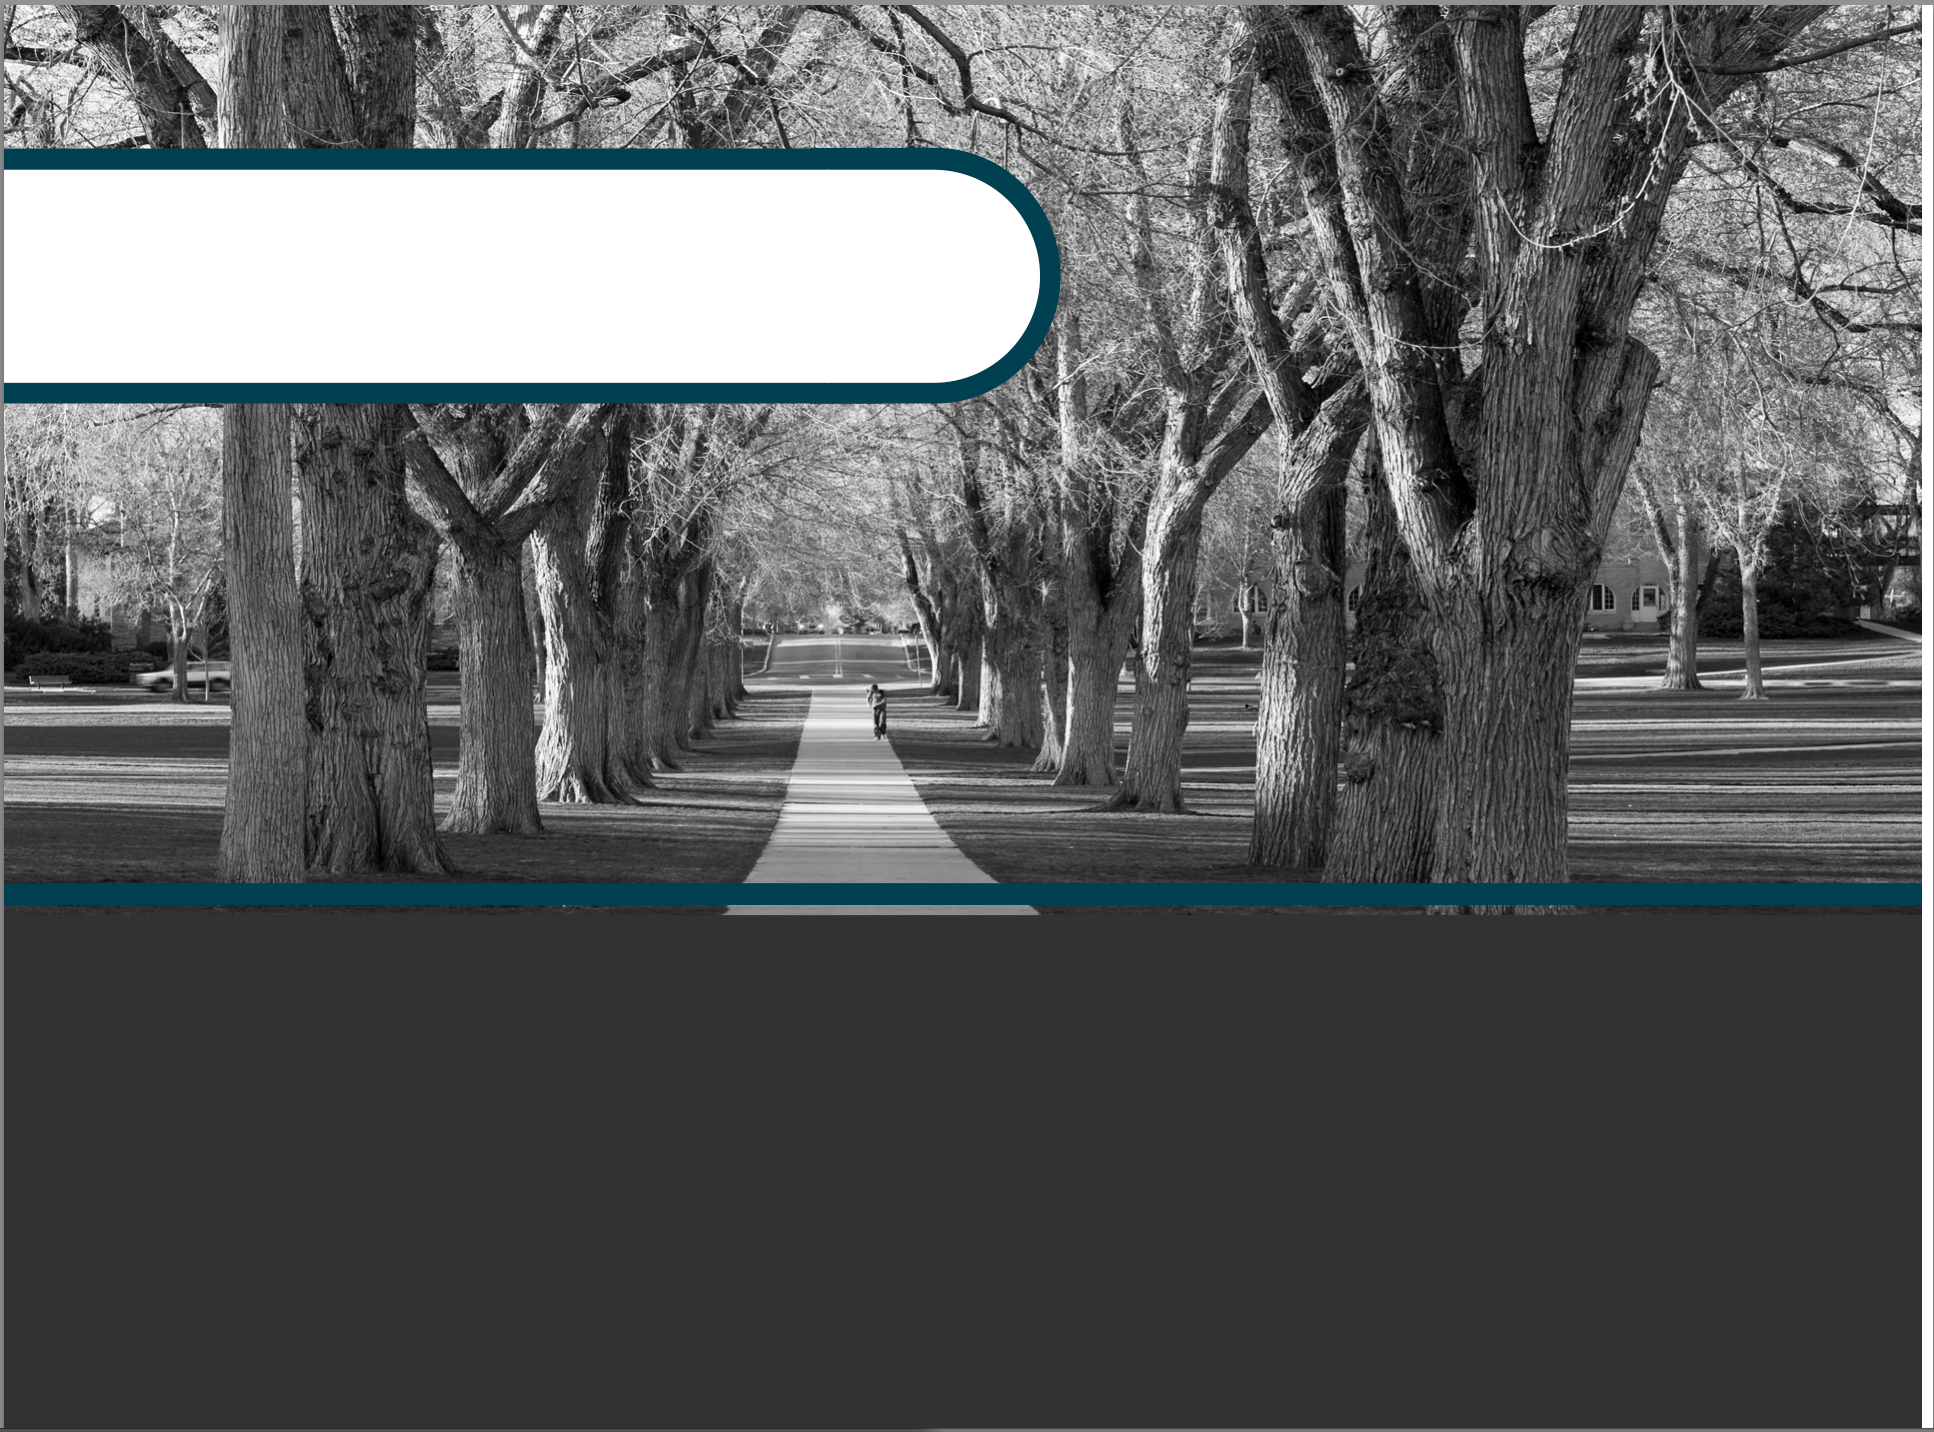
\includegraphics[width=\paperwidth]{../img/title.png}}%
\begin{frame}[plain]
  \titlepage
\end{frame}
}

\begin{frame}{Overview}
  \begin{itemize}
  \item Trainsactional or Maintenance
  \item Differences between KRAD and KNS
  \item Create a minimal transactional document that will form the basis for our Book Order document that will be used for ordering more inventory.
  \item Walk through the different steps required to build a transactional document.
  \item Learn about the different pieces that make up a transactional document.
  \end{itemize}
\end{frame}

\begin{frame}{Instructions}
 There are many steps that go into building a transactional document.  We are going to go through all of them as part of this exercise.  A basic outline of the steps that you will go through includes:
 \begin{enumerate}
   \item Create a Document object which extends TransactionalDocumentBase
   \item Create a database table to store the transactional document information.
   \item Map that table to the database using OJB.
   \end{enumerate}
\end{frame}

\begin{frame}{Instructions}
 \begin{enumerate}
   \item Create a Spring MVC Controller class that extends from TransactionalDocumentControllerBase
   \item Create a transactional document Data Dictionary file.
   \item Associate it with your Document Type
   \item Associate it with your Document class
   \item Create a KRAD View 
   \item Create and ingest a workflow DocumentType definition for your transactional document.
   \end{enumerate}
\end{frame}

\begin{frame}{Instructions}
      We will go through each of these steps to create the simplest possible Transactional Document.  Then in the next exercise we will build up the document from there to create our fully functional “Book Order” transactional document. 
\end{frame}

\begin{frame}{Get “exercise-krad-trans-doc” project}
To ensure a clean and consistent environment for everyone, we will use
the project from the USB drive as a starting point. This will
essentially be a completed copy of the previous exercises along with
some additional files to help get you started.
\end{frame}
\begin{frame}{BookOrderDocument}
\begin{enumerate}
  \item Create the BookOrderDocument Object
  \item We will create a simple BookOrderDocument object initially.  It will contain no additional attributes besides those defined on the superclass.  To do this, follow these steps:
    \begin{enumerate}
    \item Create a new package under src/main/java named train.bookstore.document
    \item Within this package, create a new class named BookOrderDocument which extends from org.kuali.rice.krad.document.TransactionalDocumentBase.
    \item Leave the class empty for now.
    \end{enumerate}
   \end{enumerate}
\end{frame}

\begin{frame}{BookOrderDocument}
\begin{enumerate}
\item Create the BookOrderDocument Database Table
  \item We have already provided the sql needed in order to create the book_order_doc_t table.
  \item Open the bookorder.sql file in the sql directory.
  \item Notice the 3 fields included in the create table statement.  These are standard columns required for all document tables:
    \begin{itemize}
      \item doc_hdr_id
      \item obj_id
      \item ver_nbr
      \end{itemize}

\begin{frame}{BookOrderDocument}
  Also notice how we don’t need to define an “_s” table to model a sequence since the doc_hdr_id is populated by the document id assigned by the Kuali Enterprise Workflow engine.  The KNS framework will handle this automatically.
\begin{enumerate}
\item Execute this sql against your database to create the book_order_doc_t table.
\item Map the book_order_doc_t table to the Database
\item Open your OJB-repository-bookstore.xml file.
\end{enumerate}
\end{frame}

\begin{frame}{BookOrderDocument}
\begin{enumerate}
\item Add an entry for the BookOrderDocument class you just created.
  This should include the following field-descriptors: 
  \begin{itemize}
  \item documentNumber -> doc_hdr_id
    \item versionNumber -> ver_nbr
    \item objectId -> obj_id
      \end{itemize}
\end{enumerate}
\end{frame}

\begin{frame}[fragile]{Add PrerequisiteConstraint}
\begin{enumerate}
    \item Include a reference-descriptor based on doc_hdr_id to point to org.kuali.rice.krad.bo.DocumentHeader.
      The mapping should resemble the following:
      \begin{minted}[fontsize=\scriptsize]{xml}
        <class-descriptor class="train.bookstore.document.BookOrderDocument" table="book_order_doc_t">
        <field-descriptor name="documentNumber" column="doc_hdr_id" jdbc-type="VARCHAR" primarykey="true" />
        <field-descriptor name="versionNumber" column="ver_nbr" jdbc-type="BIGINT" locking="true" />
        <field-descriptor name="objectId" column="obj_id" jdbc-type="VARCHAR" index="true" />
        <reference-descriptor name="documentHeader" class-ref="org.kuali.rice.krad.bo.DocumentHeader" auto-retrieve="true" auto-update="object" auto-delete="object" proxy="true" >
       	<foreignkey field-ref="documentNumber" />
        </reference-descriptor>
        </class-descriptor>
      \end{minted}
    \end{enumerate}
\end{frame}

\begin{frame}{BookOrderDocument}
We will add some more columns to this table later.  But for now, this should suffice.
\begin{enumerate}
\item  Create a new class in this package named BookOrderController which
  extends from
  org.kuali.rice.kns.web.struts.form.KualiTransactionalDocumentFormBase
\end{enumerate}
\end{frame}

\begin{frame}{Create a Transactional Document Data Dictionary File}
We have already created the skeleton for this data dictionary file for you.  Open the \textbf{BookOrderDocument.xml} file in the \textbf{src/main/resources/train/bookstore/document/datadictionary} directory.
Uncomment the body of this XML file so that both bean elements are uncommented.
\begin{enumerate} 
\item Notice how the \textbf{TransactionalDocumentEntry} associates the Document class that we created earlier with our workflow Document Type (which we will create in a later step).
\item Now open
  \textbf{src/main/resources/trnapp-BookstoreModuleBeans.xml} and add
  an entry to \textbf{dataDictionaryPackages} for your new data
  dictionary file.
\end{enumerate}


\begin{frame}{Create a Transactional Document View}
  \begin{enumerate}
  \item In contrast to Transactional Documents of old, a JSP file and
    Struts Form/Action classes/mappings are no longer necessary. By
    configuring a view with the User Interface Framework (UIF) we can
    accomplish it all within a single configuration.
  \item Once again, open \textbf{src/main/resources/train/bookstore/document/datadictionary/BookOrderDocument.xml}
    \end{enumerate}
  \end{frame}

\begin{frame}{Create a Transactional Document View}
  \begin{enumerate}
    \item Observe the following configuration.
    \begin{minted}[fontsize=\scriptsize]{xml}
<bean id="BookOrder-View" parent="Uif-TransactionalDocumentView">
  <property name="headerText" value="Book Order"/>
  <property name="formClass" value="trnapp.bookstore.BookOrderForm"/>
  <property name="documentClass" value="trnapp.bookstore.BookOrderDocument"/>
  <property name="items">
    <list>
      <ref bean="BookOrder-MainPage"/>
    </list>
  </property>
</bean>

<bean id="BookOrder-MainPage" parent="Uif-DocumentPage">
</bean>
\end{minted}
  \end{enumerate}
  \end{frame}

\begin{frame}{Create a Transactional Document View}
  \begin{enumerate}
  \item Much like the Maintenance Document, the Transactional Document
    UI is configured through its view. Now we have complete
    flexibility over it without the configuration.
  \item Transactional documents automatically map to the view using:
    \begin{minted}[fontsize=\scriptsize]{xml}
  <property name="formClass" value="trnapp.bookstore.BookOrderForm"/>
  <property name="documentClass" value="trnapp.bookstore.BookOrderDocument"/>
  \end{minted}
\item Since the Document Entry is mapped to a
  \textbf{documentTypeName}, the related \textbf{documentClass} can be
  used to query the view.
  \item Also observe that the only item in our view is a
    \textbf{Uif-DocumentPage}. This represents the structure that we
    will add elements to in further exercises.
  \end{enumerate}
\end{frame}

\begin{frame}{Create a Transactional Document View}
  \begin{enumerate}
  \item From the previous slide, you may have noticed the
    \textbf{formClass} property. This points to the Java class
    representation of what will eventually be our HTML form. KRAD
    provides an API for Transactional Document forms, but we still
    need to create one.
  \item In the \textbf{trnapp.bookstore} package, create a class
    called \textbf{BookOrderForm}
  \item Be sure to inherit from the
    \textbf{org.kuali.rice.krad.web.form.TransactionalDocumentFormBase} like below:
    \begin{minted}[fontsize=\scriptsize]{xml}
import org.kuali.rice.krad.web.form.TransactionalDocumentFormBase;

public class BookOrderForm extends TransactionalDocumentFormBase {
  \end{minted}
  \end{enumerate}
\end{frame}


  Notice how the url sends a methodToCall of “docHandler” which is a standard dispatch method that all KNS document actions support.
Create the BookOrderDocumentType
Like Maintenance Documents, Transactional Documents are also routed through the workflow engine and require a Document Type definition to be defined in the data dictionary.
To create the BookOrderDocumentType, do the following:
We have already provided you with the XML definition for the BookOrderDocumentType, you will just need to ingest it.
Launch the web application and navigate to the “XML Ingester” screen.
Browse for the file at workflow/BookOrderDocumentType.xml and click the “upload xml data” button.
This should successfully import the document type.
Test the Book Order Transactional Document
We’ve now done everything to get the very simple version of our Book Order transactional document working.  To verify this is the case, perform the following steps:
Launch the web application and navigate to the main portal page.
You should now see a link under the “Bookstore” section labeled “Book Order”.  Click on that link to create a new Book Order.
You should see a screen like the following:

This screen is not particularly exciting at the moment because we don’t have any fields on it related to a Book Order.  We’ll get to that in the next exercise.
For now, type in a description and click the “submit” button.  It should indicate that the document has been successfully submitted.
Click on the “doc search” button near the top of the portal.
When the screen loads, hit the “search” button.  You should see a result set like the following:

You can see that the document was successfully routed and has a current status of “FINAL” since no approvals were needed.

\end{document}
